%\VignetteIndexEntry{PharmacoGx: an R package for analysis of large pharmacogenomic datasets}
%\VignetteDepends{xtable}
%\VignetteSuggests{}
%\VignetteKeywords{}
%\VignettePackage{PharmacoGx}

\documentclass[11pt]{article}

\usepackage[utf8]{inputenc}
\usepackage{authblk}


\title{PharmacoGx: an R package for analysis of large pharmacogenomic datasets}
\author[1]{Petr Smirnov}
\author[1]{Zhaleh Safikhani}
\author[2]{Nehme El-Hechem}
\author[1]{Donald Wang}
\author[1]{Adrian She}
\author[1]{Catherina Olsen}
\author[1]{Mark Freeman}
\author[1]{Heather Selby}
\author[1]{Deena Gendoo}
\author[3]{Patrick Grossman}
\author[4]{Andrew Beck}
\author[3]{Hugo Aerts}
\author[1]{Mathiew Lupien}
\author[5]{Anna Goldenburg}
\author[1]{Benjamin Haibe-Kains}
\affil[1]{Princess Margaret Cancer Centre, University Health Network, Toronto Canada}
\affil[2]{Institut de recherches clinque de Montr\'{e}al, Montr\'{e}al, Canada}
\affil[3]{Dana-Farber Cancer Institute, Boston, USA}
\affil[4]{Beth Israel Deaconess Medical Center, Boston, USA}
\affil[5]{Department of Computer Science, University of Toronto, Toronto, Canada}




\usepackage{Sweave}
\begin{document}
\Sconcordance{concordance:PharmacoGx.tex:/home/chris/rPackages/PharmacoGx/vignettes/PharmacoGx.Rnw:%
1 21 1 1 4 1 1 1 0 69 1 1 3 2 0 1 1 3 0 1 2 1 1 1 2 4 0 1 2 12 1 1 3 2 %
0 1 1 3 0 1 2 5 1 1 3 5 0 1 2 16 1 1 2 1 0 3 1 1 2 1 0 1 3 2 0 1 7 4 0 %
1 5 4 0 1 6 4 0 1 5 4 0 1 6 4 0 1 5 4 0 2 1 1 5 3 0 1 4 3 0 1 4 3 0 1 3 %
1 0 1 2 1 0 1 1 1 2 1 0 1 10 13 0 1 3 2 1 1 -5 1 12 13 1 1 2 1 0 2 1 1 %
3 2 0 1 1 1 7 5 0 1 2 2 1 1 2 20 0 1 2 45 1 1 3 1 0 1 3 2 0 1 8 7 0 1 8 %
7 0 4 1 16 0 1 2 51 1 1 2 31 0 1 2 4 1}


\maketitle
\tableofcontents

%------------------------------------------------------------
\section{Introduction}
%------------------------------------------------------------

Pharmacogenomics hold much potential to aid in discovering drug response
biomarkers and developing novel targeted therapies, leading to development of
precision medicine and working towards the goal of personalized therapy.
Several large experiments have been conducted, both to molecularly
characterize drug dose response across many cell lines, and to examine the
molecular response to drug administration. However, the experiments lack a
standardization of protocols and annotations, hindering meta-analysis across
several experiments.\\

\textit{PharmacoGx} was developed to address these challenges, by providing a
unified framework for downloading and analyzing large pharmacogenomic datasets
which are extensively curated to ensure maximum overlap and consistency.
\textit{PharmacoGx} is based on a level of abstraction from the raw
experimental data, and allows bioinformaticians and biologists to work with
data at the level of genes, drugs and cell lines. This provides a more
intuitive interface and, in combination with unified curation, simplifies
analyses between multiple datasets.\\

To organize the data released by each experiment, we developed the
\textit{PharmacoSet} class. This class efficiently stores different types of
data and facilitates interrogating the data by drug or cell line. The
\textit{PharmacoSet} is also versatile in its ability to deal with two
distinct types of pharmacogenomic datasets. The first type, known as
\textit{sensitivity} datasets, are datasets where cell lines were profiled
on the molecular level, and then tested for drug dose response. The second
type of dataset is the \textit{perturbation} dataset. These types of
datasets profile a cell line on the molecular level before and after
administration of a compound, to characterize the action of the compound on
the molecular level.\\

With the first release of \textit{PharmacoGx} we have fully curated and
created PharmacoSet objects for three publicly available large pharmacogenomic
datasets. Two of these datasets are of the \textit{sensitivity} type. These
are the Cancer Genome Project (CGP) \cite{Garnett:2012fc} and the Cancer Cell
Line Encyclopedia (CCLE) \cite{Barretina:2012fp}. The third dataset is of the
\textit{perturbation} type, the Connectivity Map (CMAP) project
\cite{Lamb:2006hf}.\\

Furthermore, PharmacoGx provides a suite of parallized functions which
facilitate drug response biomarker discovery, and molecular drug
characterization. This vignette will provide two example analysis case
studies. The first will be comparing gene expression and drug sensitivity
measures across the CCLE and CGP projects. The second case study will
interrogate the CMAP database with a known signature of up and down regulated
genes for HDAC inhibitors as published in ~\cite{Glaser:2003gk}. Using the
Connectivity Score as defined in ~\cite{Lamb:2006hf}, it will be seen that
known HDAC inhibitors have a high numerical score and high significance.\\ %%'check if the reference is right

For the purpose of this vignette, an extremely minuscule subset of all three
\textit{PharmacoSet} objects are included with the package as example data.
They are included for illustrative purposes only, and the results obtained
with them will likely be meaningless.\\


%------------------------------------------------------------
\subsection{Installation and Settings}
%------------------------------------------------------------

\textit{PharmacoGx} requires that several packages are installed. However, all dependencies are available from CRAN or Bioconductor.

\begin{Schunk}
\begin{Sinput}
> source('http://bioconductor.org/biocLite.R')
> biocLite('PharmacoGx')
\end{Sinput}
\end{Schunk}

Load \textit{PharamacoGx} into your current workspace:
\begin{Schunk}
\begin{Sinput}
> library(PharmacoGx)
\end{Sinput}
\end{Schunk}

%------------------------------------------------------------
\subsection{Requirements}
%------------------------------------------------------------

\textit{PharmacoGx} has been tested on Windows, Mac and Cent OS platforms.

The packages uses the core R package \textit{parallel} to preform parallel computations, and therefore if parallelization is desired, the dependencies for the parallel package must be met. 

%------------------------------------------------------------
\section{Downloading PharmacoSet objects}
%------------------------------------------------------------

We have made the PharmacoSet objects of the curated datasets available online at:\\ \textit{www.pmgenomics.ca/bhklab/software/pharmacogx/}\\
However, to make the process of obtaining the data easier through the R shell, we have also written a function \textit{downloadPSet} which automates downloading the datasets into a directory of the users choice, and returns the data into the R session. 

\begin{Schunk}
\begin{Sinput}
> ## Example
> CGP <- downloadPSet('CGP') 
\end{Sinput}
\end{Schunk}
%------------------------------------------------------------
\subsection{Downloading Drug Signatures}
%------------------------------------------------------------

The package also provides tools to compute drug perturbation and sensitivity signatures, as explained below. However, this computation is lengthy, so for users convenience we have precomputed signatures for our three PharmacoSet objects and made them available for download using the function \textit{downloadSignatures}.

\begin{Schunk}
\begin{Sinput}
> ## Example
> CGP.sigs <- downloadSignatures('CGP')
\end{Sinput}
\end{Schunk}

%------------------------------------------------------------
\section{Sensitivity Case Study}
%------------------------------------------------------------

Our first case study illustrates the functions for analysis of the \textit{sensitivity} type of dataset. The case study will investigate the consistency between the CGP and CCLE datasets, recreating the analysis similar to our \textit{Inconsistency in Large Pharmacogenomic Studies} paper \cite{HaibeKains:2013ie}. In both CCLE and CGP, the transcriptome of cells was profiled using an Affymatrix microarray chip. Cells were also tested for their response to increasing concentrations of various compounds, and form this the IC50 and AUC were computed. However, the cell and drugs names used between the two datasets were not consistent. Furthermore, two different microarray platforms were used. However, \textit{PharmacoGx} allows us to overcome these differences to do a comparative study between these two datasets. \\


CGP was profiled using the hgu133a platform, while CCLE was profiled with the expanded hgu133plus2 platform. While in this case the hgu133a is almost a strict subset of hgu133plus2 platform, we can use the best information from each platform by comparing the best probes within each dataset per gene. The function \textit{probeGeneMapping} selects a probe for each gene profiled in the microarray platform. It picks the most accurate probe for each gene using annotations extracted from the jetset package \cite{Li:2011cc}. Jetset scores each probe on how sensitive and specific it is, allowing probeGeneMapping to pick the probe which is most representative of each genes true expression. \\

To begin, you would load the datasets from disk or download them using the \textit{downloadPSet} function above, and then execute probeGeneMapping on the datasets. 

\begin{Schunk}
\begin{Sinput}
>   ##Using the included example datasets
>   library(PharmacoGx)
>   data("CGPsmall")
>   data("CCLEsmall")
>   CGPsmall <- probeGeneMapping(CGPsmall) 
>   CCLEsmall <- probeGeneMapping(CCLEsmall) 
\end{Sinput}
\end{Schunk}
We then want to investigate the consistency of the data between the two datasets. The common intersection between the datasets can then be found using \textit{intersectPSet}. We then create a summary of the gene expression and drug sensitivity measures for both datasets, and compare them using a standard correlation coefficient. 

\begin{Schunk}
\begin{Sinput}
>   library(PharmacoGx)
>   data("CGPsmall")
>   data("CCLEsmall")
>   CGPsmall <- probeGeneMapping(CGPsmall) 
>   CCLEsmall <- probeGeneMapping(CCLEsmall) 
>   common <- intersectPSet(list('CCLE'=CCLEsmall,
+                                'CGP'=CGPsmall),
+                           intersectOn=c("cell.lines", "drugs", 'genes'))
>   CGP.auc <- summarizeSensitivityPhenotype(
+                 common$CGP, 
+                 sensitivity.measure='auc_published', 
+                 summaryStat="median")
>   CCLE.auc <- summarizeSensitivityPhenotype(
+                 common$CCLE, 
+                 sensitivity.measure='auc_published', 
+                 summaryStat="median")
>   CGP.ic50 <- summarizeSensitivityPhenotype(
+                 common$CGP, 
+                 sensitivity.measure='ic50_published', 
+                 summaryStat="median")
>   CCLE.ic50 <- summarizeSensitivityPhenotype(
+                 common$CCLE, 
+                 sensitivity.measure='ic50_published', 
+                 summaryStat="median")
>   common$CGP <- summarizeGeneExpression(common$CGP, 
+                                         cellNames(common$CGP),
+                                         verbose=FALSE)
>   common$CCLE <- summarizeGeneExpression(common$CCLE, 
+                                          cellNames(common$CCLE),
+                                          verbose=FALSE)
>   gg <- geneNames(common[[1]])
>   cc <- cellNames(common[[1]])
>   ge.cor <- sapply(cc, function (x, d1, d2) {
+     return (cor(d1[ , x], d2[ , x], method="spearman",
+                 use="pairwise.complete.obs"))
+   }, d1=rnaData(common$CGP), d2=rnaData(common$CCLE))
>   ic50.cor <- sapply(cc, function (x, d1, d2) {
+     return (cor(d1[, x], d2[ , x], method="spearman",
+                 use="pairwise.complete.obs"))
+   }, d1=t(CGP.ic50), d2=t(CCLE.ic50))
>   auc.cor <- sapply(cc, function (x, d1, d2) {
+     return (cor(d1[ , x], d2[ , x], method="spearman",
+                 use="pairwise.complete.obs"))
+   }, d1=t(CGP.auc), d2=t(CCLE.auc))
>   w1 <- wilcox.test(x=ge.cor, y=auc.cor, conf.int=TRUE)
>   w2 <- wilcox.test(x=ge.cor, y=ic50.cor, conf.int=TRUE)
>   yylim <- c(-1, 1)
>   ss <- sprintf("GE vs. AUC = %.1E\nGE vs. IC50 = %.1E",
+                 w1$p.value, w2$p.value)
>   boxplot(list("GE"=ge.cor, "AUC"=auc.cor, "IC50"=ic50.cor),
+           main="Concordance between cell lines",
+           ylab=expression(R[s]),
+           sub=ss,
+           ylim=yylim,
+           col="lightgrey",
+           pch=20,
+           border="black")
> 
\end{Sinput}
\end{Schunk}

\begin{figure}[H!]
\begin{center}
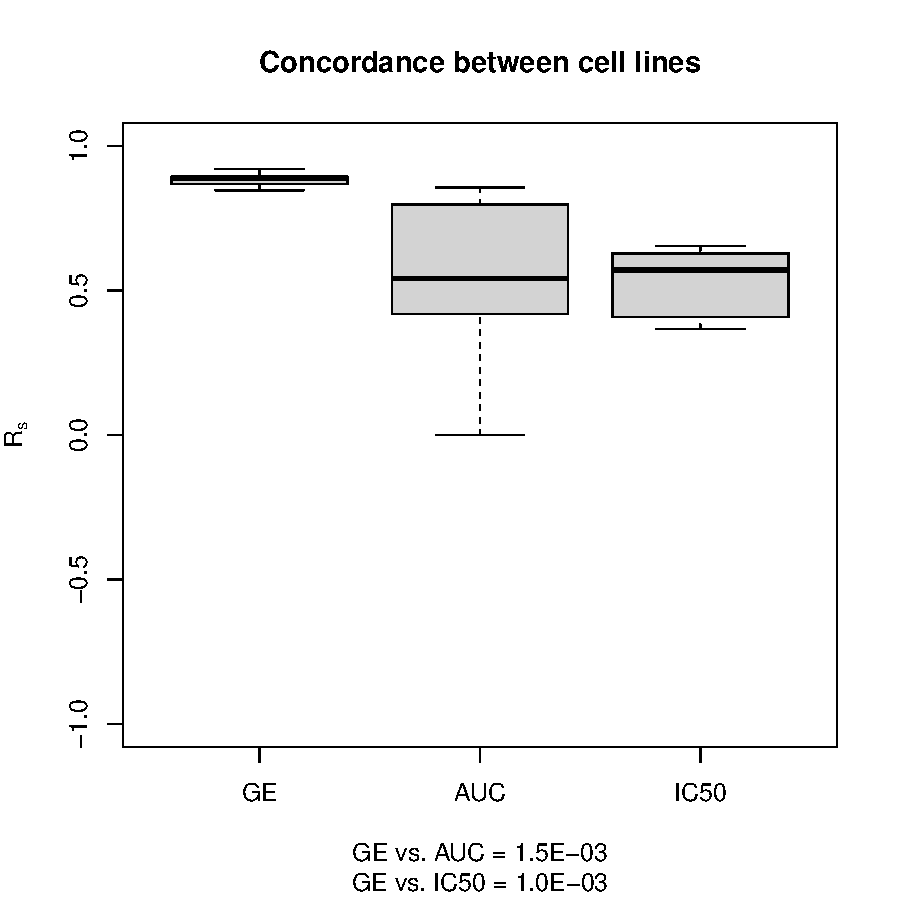
\includegraphics{PharmacoGx-fig2}
\end{center}
\label{fig:one}
\end{figure}

%------------------------------------------------------------
\section{Perturbation Case Study}
%------------------------------------------------------------

The second case study illustrates the analysis of a perturbation type datasets, where the changes in cellular molecular profiles are compared before and after administering a compound to the cell line. Of these datasets, we have currently curated and made available for download the Connectivity Map (CMAP) dataset \cite{Lamb:2006hf}. \\

For this case study, we will recreate an analysis from the paper by Lamb et al., in which a known signature for HDAC inhibitors \cite{Glaser:2003gk} is used to recover drugs in the CMAP dataset that are also known HDAC inhibitors. For this example, the package includes this signature, already mapped to the gene level, and it can be loaded by calling \textit{data(HDAC\_genes)}.

Once again, we load the dataset, and we summarize the expression on the gene level using \textit{probeGeneMapping}. We then recreate drug signatures for each drug use the function \textit{drugPerturbationSig} to preform statistical modelling of the transcriptomic response to the application of each drug. We then compare the observed upregulated and downregulated genes to a the known HDAC signature, using the GSEA connectivity score to determine the correlation between the two signatures. 

\begin{Schunk}
\begin{Sinput}
>   library(PharmacoGx)
>   require(xtable)
>   data(CMAPsmall)
>   drug.perturbation <- drugPertubrationSig(CMAPsmall)
>   data(HDAC_genes)
>   res <- apply(drug.perturbation[,,c("tstat", "fdr")], 2, function(x, HDAC){ 
+ 	    return(connectivityScore(x=x, 
+ 	                             y=HDAC[,2,drop=FALSE], 
+ 	                             method="gsea", nperm=100))
+ 	}, HDAC=HDAC_genes)
>   rownames(res) <- c("Connectivity", "P Value")
>   res <- t(res)
>   res <- res[order(res[,1], decreasing=T),]
>   xtable(res, 
+     caption='Connectivity Score results for HDAC inhibitor gene signature.')
\end{Sinput}
% latex table generated in R 3.2.1 by xtable 1.7-4 package
% Tue Jul 21 22:02:12 2015
\begin{table}[ht]
\centering
\begin{tabular}{rrr}
  \hline
 & Connectivity & P Value \\ 
  \hline
vorinostat & 0.99 & 0.00 \\ 
  alvespimycin & 0.82 & 0.00 \\ 
  acetylsalicylic acid & 0.50 & 0.33 \\ 
  rosiglitazone & 0.00 & 1.00 \\ 
  pioglitazone & 0.00 & 1.00 \\ 
   \hline
\end{tabular}
\caption{Connectivity Score results for HDAC inhibitor gene signature.} 
\end{table}\end{Schunk}
As we can see, the known HDAC inhibitor Varinostat has a very strong connectivity score, as well as a very high significance as determined by permutation testing, in comparison to the other drugs, which score poorly. 

This example serves as a validation of the method, and demonstrates the ease with which drug perturbation analysis can be done using \textit{PharmacoGx}. While in this case we were matching a drug signature with a drug class signature, this method can also be used in the discovery of drugs that are anticorrelated with known disease signatures, to look for potential new treatments and drug repurposing. 
%------------------------------------------------------------
\section{Session Info}
%------------------------------------------------------------ 

\begin{itemize}\raggedright
  \item R version 3.2.1 Patched (2015-07-08 r68642), \verb|x86_64-apple-darwin13.4.0|
  \item Locale: \verb|en_CA.UTF-8/en_CA.UTF-8/en_CA.UTF-8/C/en_CA.UTF-8/en_CA.UTF-8|
  \item Base packages: base, datasets, graphics, grDevices, methods,
    stats, utils
  \item Other packages: PharmacoGx~1.0.3, xtable~1.7-4
  \item Loaded via a namespace (and not attached): Biobase~2.29.1,
    BiocGenerics~0.15.3, bitops~1.0-6, caTools~1.17.1, cluster~2.0.2,
    digest~0.6.8, downloader~0.4, gdata~2.17.0, gplots~2.17.0,
    gtools~3.5.0, igraph~1.0.1, KernSmooth~2.23-15, limma~3.25.13,
    magicaxis~1.9.4, magrittr~1.5, marray~1.47.0, MASS~7.3-42,
    parallel~3.2.1, piano~1.9.4, plotrix~3.5-12, RColorBrewer~1.1-2,
    relations~0.6-5, sets~1.0-15, slam~0.1-32, sm~2.2-5.4, tools~3.2.1
\end{itemize}
\bibliographystyle{plain}
\bibliography{biblio}

\end{document}
